Die stochastische Kodierung nutzt ein zufällig generiertes Muster als Szene.
Geeignet für dieses Verfahren sind sogenannte \glqq Specklemuster\grqq ~\cite{specklePattern}.
Es handelt sich dabei um bandbegrenzte Muster mit zufällig verteilten Grauwerten.
Aufgrund der Unschärfe und dem Rauschen, welche in der Aufnahme durch eine Kamera einfließen, ist die Bandbegrenztheit notwendig um eine Dekodierung zu ermöglichen.
Abbildung \ref{img:speckleMuster} zeigt ein solches Muster.
%
\begin{figure}[H]
	\centering
	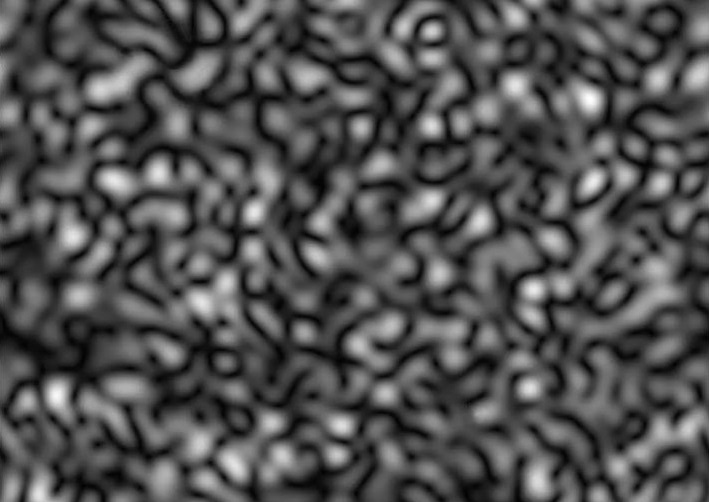
\includegraphics[frame,width=0.5\textwidth]{02_grundlagenZurDeflektometrie/rekonstruktion/stochastischeKodierung/figures/speckleMuster}
	\caption[Specklemuster]{Specklemuster.}
	\label{img:speckleMuster}
\end{figure}
%
Das Prinzip sieht drei Aufnahmen unter Beobachtung des erzeugten Specklemusters vor.
Zunächst eine Aufnahme des Prüfobjekts bei Spiegelung des Specklemusters.
Dann wird das Specklemuster in der $x$-Richtung verschoben und aufgenommen.
Dasselbe wird auch mit der Verschiebung in $y$-Richtung 